% Template for PLoS
% Version 3.1 February 2015
%
% To compile to pdf, run:
% latex plos.template
% bibtex plos.template
% latex plos.template
% latex plos.template
% dvipdf plos.template
%
% % % % % % % % % % % % % % % % % % % % % %
%
% -- IMPORTANT NOTE
%
% This template contains comments intended 
% to minimize problems and delays during our production 
% process. Please follow the template instructions
% whenever possible.
%
% % % % % % % % % % % % % % % % % % % % % % % 
%
% Once your paper is accepted for publication, 
% PLEASE REMOVE ALL TRACKED CHANGES in this file and leave only
% the final text of your manuscript.
%
% There are no restrictions on package use within the LaTeX files except that 
% no packages listed in the template may be deleted.
%
% Please do not include colors or graphics in the text.
%
% Please do not create a heading level below \subsection. For 3rd level headings, use \paragraph{}.
%
% % % % % % % % % % % % % % % % % % % % % % %
%
% -- FIGURES AND TABLES
%
% Please include tables/figure captions directly after the paragraph where they are first cited in the text.
%
% DO NOT INCLUDE GRAPHICS IN YOUR MANUSCRIPT
% - Figures should be uploaded separately from your manuscript file. 
% - Figures generated using LaTeX should be extracted and removed from the PDF before submission. 
% - Figures containing multiple panels/subfigures must be combined into one image file before submission.
% For figure citations, please use "Fig." instead of "Figure".
% See http://www.plosone.org/static/figureGuidelines for PLOS figure guidelines.
%
% Tables should be cell-based and may not contain:
% - tabs/spacing/line breaks within cells to alter layout or alignment
% - vertically-merged cells (no tabular environments within tabular environments, do not use \multirow)
% - colors, shading, or graphic objects
% See http://www.plosone.org/static/figureGuidelines#tables for table guidelines.
%
% For tables that exceed the width of the text column, use the adjustwidth environment as illustrated in the example table in text below.
%
% % % % % % % % % % % % % % % % % % % % % % % %
%
% -- EQUATIONS, MATH SYMBOLS, SUBSCRIPTS, AND SUPERSCRIPTS
%
% IMPORTANT
% Below are a few tips to help format your equations and other special characters according to our specifications. For more tips to help reduce the possibility of formatting errors during conversion, please see our LaTeX guidelines at http://www.plosone.org/static/latexGuidelines
%
% Please be sure to include all portions of an equation in the math environment.
%
% Do not include text that is not math in the math environment. For example, CO2 will be CO\textsubscript{2}.
%
% Please add line breaks to long display equations when possible in order to fit size of the column. 
%
% For inline equations, please do not include punctuation (commas, etc) within the math environment unless this is part of the equation.
%
% % % % % % % % % % % % % % % % % % % % % % % % 
%
% Please contact latex@plos.org with any questions.
%
% % % % % % % % % % % % % % % % % % % % % % % %

\documentclass[10pt,letterpaper]{article}
\usepackage[top=0.85in,left=2.75in,footskip=0.75in]{geometry}

% Use adjustwidth environment to exceed column width (see example table in text)
\usepackage{changepage}

% Use Unicode characters when possible
\usepackage[utf8]{inputenc}

% textcomp package and marvosym package for additional characters
\usepackage{textcomp,marvosym}

% fixltx2e package for \textsubscript
\usepackage{fixltx2e}

% amsmath and amssymb packages, useful for mathematical formulas and symbols
\usepackage{amsmath,amssymb}

% cite package, to clean up citations in the main text. Do not remove.
\usepackage{cite}

% Use nameref to cite supporting information files (see Supporting Information section for more info)
\usepackage{nameref,hyperref}

% line numbers
\usepackage[right]{lineno}

% ligatures disabled
\usepackage{microtype}
\DisableLigatures[f]{encoding = *, family = * }

% rotating package for sideways tables
\usepackage{rotating}

% Remove comment for double spacing
%\usepackage{setspace} 
%\doublespacing

% Text layout
\raggedright
\setlength{\parindent}{0.5cm}
\textwidth 5.25in 
\textheight 8.75in

% Bold the 'Figure #' in the caption and separate it from the title/caption with a period
% Captions will be left justified
\usepackage[aboveskip=1pt,labelfont=bf,labelsep=period,justification=raggedright,singlelinecheck=off]{caption}

% Use the PLoS provided BiBTeX style
\bibliographystyle{plos2015}

% Remove brackets from numbering in List of References
\makeatletter
\renewcommand{\@biblabel}[1]{\quad#1.}
\makeatother

% Leave date blank
\date{}

% Header and Footer with logo
\usepackage{lastpage,fancyhdr,graphicx}
\usepackage{epstopdf}
\pagestyle{myheadings}
\pagestyle{fancy}
\fancyhf{}
\lhead{
\includegraphics[width=2.0in]{PLOS-submission.eps}}
\rfoot{\thepage/\pageref{LastPage}}
\renewcommand{\footrule}{\hrule height 2pt \vspace{2mm}}
\fancyheadoffset[L]{2.25in}
\fancyfootoffset[L]{2.25in}
\lfoot{\sf PLOS}

%% Include all macros below

\newcommand{\lorem}{{\bf LOREM}}
\newcommand{\ipsum}{{\bf IPSUM}}

%% END MACROS SECTION


\begin{document}
\vspace*{0.35in}

% Title must be 250 characters or less.
% Please capitalize all terms in the title except conjunctions, prepositions, and articles.
\begin{flushleft}
{\Large
\textbf\newline{MC-Cons: RNA secondary structural assignments}
}
\newline
% Insert author names, affiliations and corresponding author email (do not include titles, positions, or degrees).
\\
Gabriel C-Parent, % \textsuperscript{1},
Francois Major%\textsuperscript{1},
%with the Lorem Ipsum Consortium\textsuperscript{\textpilcrow}
\\
\bigskip
%\bf{1} 
Institute for Research in Immunology and Cancer, and Department of Computer Science, Université de Montréal, Montreal, QC, H3C 3J7, Canada
%\\
%\bf{2} Affiliation Dept/Program/Center, Institution Name, City, State, Country
%\\
%\bf{3} Affiliation Dept/Program/Center, Institution Name, City, State, Country
\\
\bigskip

% Insert additional author notes using the symbols described below. Insert symbol callouts after author names as necessary.
% 
% Remove or comment out the author notes below if they aren't used.
%
% Primary Equal Contribution Note
%\Yinyang These authors contributed equally to this work.
%
%% Additional Equal Contribution Note
%% Also use this double-dagger symbol for special authorship notes, such as senior authorship.
%\ddag These authors also contributed equally to this work.
%
%% Current address notes
%\textcurrency a Insert current address of first author with an address update
%% \textcurrency b Insert current address of second author with an address update
%% \textcurrency c Insert current address of third author with an address update
%
%% Deceased author note
%\dag Deceased
%
%% Group/Consortium Author Note
%\textpilcrow Membership list can be found in the Acknowledgments section.
%
%% Use the asterisk to denote corresponding authorship and provide email address in note below.
* gabriel.c-parent@umontreal.ca

\end{flushleft}
% Please keep the abstract below 300 words


% WHAT KIND OF ARTICLE? : software paper right? although it's more algorithm with implementation given

\section*{Abstract}

We consider the problem of selecting 
RNA secondary structural assignment is an interesting problem. Bla bla bla.


% Please keep the Author Summary between 150 and 200 words
% Use first person. PLOS ONE authors please skip this step. 
% Author Summary not valid for PLOS ONE submissions.

\section*{Author Summary}
%Despite the clear functional importance of structure in RNA molecules, it remains very difficult to correctly identify and annotate similar RNA structures because their sequences are often poorly conserved even for RNAs that form very similar higher-order structures. A solution is to use a metric that identifies structural motifs but this, too, is difficult because RNA structure modeling based on sequence alone is generally not very accurate. In this work, we use SHAPE chemical probing to obtain model-free information about RNA structure and then exploit this information to align RNAs by sequence. We show for ribosomal RNAs that sequence alignments based on SHAPE experimental information alone are as accurate as those that actually use sequence information. In addition, we identify regions in the 16S ribosomal RNA that form conserved secondary structures that are different from currently accepted models. These differences, rather than being errors, reveal sites of conformational flexibility that may underlie mechanistic functions in ribosome assembly and translation regulation. We anticipate that structure-informed sequence alignment and structure modeling will become broadly useful tools in RNA function analysis.

\linenumbers

\section*{Introduction}

% context

%Lorem ipsum dolor %sit~\cite{bib1}%%
%amet, consectetur adipiscing elit. Curabitur eget porta erat. Morbi consectetur est vel gravida pretium. Suspendisse ut dui eu ante cursus gravida non sed sem. Nullam Eq.~(\ref{eq:schemeP}) sapien tellus, commodo id velit id, eleifend volutpat quam. Phasellus mauris velit, dapibus finibus elementum vel, pulvinar non tellus. Nunc pellentesque pretium diam, quis maximus dolor faucibus id. Nunc convallis sodales ante, ut ullamcorper est egestas vitae. Nam sit amet enim ultrices, ultrices elit pulvinar, volutpat risus.

%\begin{equation}\label{eq:schemeP} 
%D_{coll} = \frac{D_f+\frac{[S]^2}{K_D S_T} D_S} {1+\frac{[S]^2}{K_D S_T}}, 
%D_{sm} = \frac{D_f+ \frac{[S]}{K_D} D_S}{1+\frac{[S]}{K_D}},
%\end{equation}





% You may title this section "Methods" or "Models". 
% "Models" is not a valid title for PLoS ONE authors. However, PLoS ONE
% authors may use "Analysis"
\newpage
\section*{Design and Implementation}

\subsection*{Consensus Problem}

Given $n$ sets of $ m_1, m_2... m_n$ objects, the consensus problem is to find a set of $n$ objects, one per set, minimizing the sum of their pairwise distance.

\noindent The consensus problem can be transformed into a MIN-SUM \textit{compact location problem} \cite{compact_location}. To reduce it, we add a large positive penalty $M$ to the distance of objects belonging to the same set. This way, any consensus using more than one object belonging to the same set is noncompetitive. Since the MIN-SUM compact location problem is NP-HARD, even for metric distance functions \cite{compact_location}, the use of heuristics is justified.



% introduce the problem

% sp-alignment

% introduce compact location problem
% basic properties
%\noindent Naively, given $n$ molecules each with $m$ secondary structures, the going through the full search space would involve the evaluation of $m^n$ solutions. This is obviously not a good ideaHowever, the idea of 

%Minimizing the sum of pairwise distance between sets of objects has been extensively investigated in the field of location theory \cite{compact_location}. Indeed, each step of the \newline
%
%
%% mapping of the consensuss problem to the compact location problem by
%% tweaking the distance function using infinity as intra group distance
%% may need more details to proove it, let's see what Francois thinks
%\noindent The consensus problem described here can be reduced to an instance of the minimum average distance placement (MIN-SUM) by modifying the distance function in use such that elements belonging to the same group have infinite distance, thereby guaranteeing that a consensus will never contain more than one element of each group. This convenient reduction allows us to benefit from previously derived hardness results and justify the use of meta-heuristics.
%
%\noindent Using a metric distance function, one might think that it would be possible to reduce efficiently the search space, but even finding a near-optimal placement within a certain factor of the optimal has been proved to be NP-Hard \cite{compact_location}.



\subsection*{RNA Secondary Structure and the Consensus Problem}

Most RNA secondary structure prediction tools allow for the exploration of suboptimal secondary structures. Very often, the experimentally determined structures of reference structures can be found close to the best structure found.

When working with functionally related RNAs such as Iron Response Elements (IREs) or transfer RNAs (tRNAs), one might expect that the function can be explained by some, potentially many, shared structures. To this end, our goal was to devise a method capable of finding similar structures
%citer l'article de mc-fold et Paul

MC-Cons is a two-step optimization procedure (Fig.~\ref{fig1}). The first step is to create consensus of base pair trees using a tree edit distance function to compare them. This step insures that the overall topology of stems in the structures of the consensus is as similar as possible. The second step refines the consensus previously created by minimizing the string edit distance on the Vienna dot-bracket representation of RNA secondary structure. This step insures that unpaired regions match as well as possible.



\begin{figure}[h]
\begin{center}
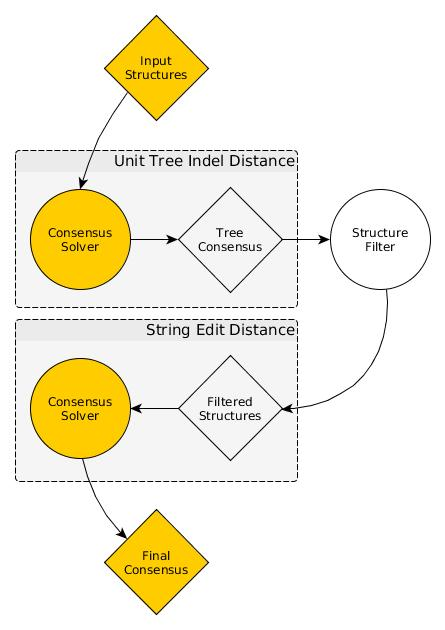
\includegraphics[scale=0.4]{figs/mccons_flowchart2.eps}
\caption{{\bf Flowchart illustration of MC-Cons}
The two-step procedure is simple. Its input is a marna-like formatted file of RNA sequences and secondary structures in Vienna dot-bracket format. Its output is a marna-like formatted  The two main optimization steps are highlighted in grey.}
\label{fig1}
\end{center}
\end{figure}


\subsection*{Base Pair Trees and Unit Tree Indel Distance}
% base pair tree representation vs abstract shapes
% upsides and downsides of the
% representation compared to abstract shape
We define base pair trees as ordered rooted trees built from the base pairs of a RNA secondary structure. This representation is similar to the RNA abstract shapes level 5 \cite{abstract_shapes} with the added benefit that it preserve stems length information.


% relation to the tree edit distance (special scoring scheme)
\noindent To compare such trees, we use a standard tree edit distance \cite{zhang_shasha} along with a custom scoring scheme to compare base pair trees. Under this scoring scheme, insertions and deletions have unit cost.

% interpretation of a score
\noindent This distance function is intuitive. A distance of $n$ between two base pair trees means that it is possible to convert each tree into the other with a minimum of $n$ modifications (insertions and deletions of base pairs).

%Notice that the distance function retains the metric properties (non-negativity, symmetry, subadditivity).







\subsection*{Consensus Solvers}
% complexity justifies meta-heuristic
Given the complexity of the consensus problem, the use of heuristics is well justified. We still give an exact solver.

% check which details should be given, keep it as simple as possible
% article using metaheuristics? stuff from class maybe?

% mention the interface, the solvers are given a precomputed distance matrix!
\noindent Many simple heuristics were found to perform well within reasonable time. These algorithms all take precomputed distance matrices whose calculation is embarrassingly parallel.

% for the article, we'll ignore the steepest descent solver for now, it is useless
% version 1: Exact Version (branch & bound)
\paragraph{Exact Version: Branch \& Bound}
First, an exact version of the consensus solver based on a branch \& bound design was created to compare the performance of different heuristics on small instances.

\noindent The lower bound of an incomplete solution is estimated by the summation of pairwise distances between the chosen objects and the best distance they have to remaining sets of objects to be chosen. This bound is generally quite good on small instances, but its performance degrades rapidly as the number of molecules grows.

% version 2: Genetic Algorithm
\paragraph{Heuristic: Genetic Algorithm}
The genetic algorithm solver uses generic mutation (random substitution) and crossover operators (uniform) along with elitist selection. To increase convergence rate, an improvement operator using a steepest descent procedure is used.

\noindent The local search is done by finding the substitution which improves the most the current sum of pairs distance. The operator applies a small number of iterations of local search with a certain probability.







\newpage

% For figure citations, please use "Fig." instead of "Figure".
%Nulla mi mi, Fig.~\ref{fig1} venenatis sed ipsum varius, volutpat euismod diam. Proin rutrum vel massa non gravida. Quisque tempor sem et dignissim rutrum. Lorem ipsum dolor sit amet, consectetur adipiscing elit. Morbi at justo vitae nulla elementum commodo eu id massa. In vitae diam ac augue semper tincidunt eu ut eros. Fusce fringilla erat porttitor lectus cursus, \nameref{S1_Video} vel sagittis arcu lobortis. Aliquam in enim semper, aliquam massa id, cursus neque. Praesent faucibus semper libero.



%\begin{enumerate}
%\item{react}
%\item{diffuse free particles}
%\item{increment time by dt and go to 1}
%\end{enumerate}

% Results and Discussion can be combined.
\newpage
\section*{Results}

To demonstrate the performance of MC-Cons, 
Nulla mi mi, venenatis sed ipsum varius, Table~\ref{table1} volutpat euismod diam. Proin rutrum vel massa non gravida. Quisque tempor sem et dignissim rutrum. Lorem ipsum dolor sit amet, consectetur adipiscing elit. Morbi at justo vitae nulla elementum commodo eu id massa. In vitae diam ac augue semper tincidunt eu ut eros. Fusce fringilla erat porttitor lectus cursus, vel sagittis arcu lobortis. Aliquam in enim semper, aliquam massa id, cursus neque. Praesent faucibus semper libero.


\begin{table}[!ht]
\begin{adjustwidth}{-2.25in}{0in} % Comment out/remove adjustwidth environment if table fits in text column.
\caption{
{\bf Table caption Nulla mi mi, venenatis sed ipsum varius, volutpat euismod diam.}}
\begin{tabular}{|l|l|l|l|l|l|l|l|}
\hline
\multicolumn{4}{|l|}{\bf Heading1} & \multicolumn{4}{|l|}{\bf Heading2}\\ \hline
$cell1 row1$ & cell2 row 1 & cell3 row 1 & cell4 row 1 & cell5 row 1 & cell6 row 1 & cell7 row 1 & cell8 row 1\\ \hline
$cell1 row2$ & cell2 row 2 & cell3 row 2 & cell4 row 2 & cell5 row 2 & cell6 row 2 & cell7 row 2 & cell8 row 2\\ \hline
$cell1 row3$ & cell2 row 3 & cell3 row 3 & cell4 row 3 & cell5 row 3 & cell6 row 3 & cell7 row 3 & cell8 row 3\\ \hline
\end{tabular}
\begin{flushleft} Table notes Phasellus venenatis, tortor nec vestibulum mattis, massa tortor interdum felis, nec pellentesque metus tortor nec nisl. Ut ornare mauris tellus, vel dapibus arcu suscipit sed.
\end{flushleft}
\label{table1}
\end{adjustwidth}
\end{table}



\subsection*{\lorem\ and \ipsum\ Nunc blandit a tortor.}

Maecenas convallis mauris sit amet sem ultrices gravida. Etiam eget sapien nibh. Sed ac ipsum eget enim egestas ullamcorper nec euismod ligula. Curabitur fringilla pulvinar lectus consectetur pellentesque. Quisque augue sem, tincidunt sit amet feugiat eget, ullamcorper sed velit. Sed non aliquet felis. Lorem ipsum dolor sit amet, consectetur adipiscing elit. Mauris commodo justo ac dui pretium imperdiet. Sed suscipit iaculis mi at feugiat. 

\subsection*{Sed ac quam id nisi malesuada congue.}

Nulla mi mi, venenatis sed ipsum varius, volutpat euismod diam. Proin rutrum vel massa non gravida. Quisque tempor sem et dignissim rutrum. Lorem ipsum dolor sit amet, consectetur adipiscing elit. Morbi at justo vitae nulla elementum commodo eu id massa. In vitae diam ac augue semper tincidunt eu ut eros. Fusce fringilla erat porttitor lectus cursus, vel sagittis arcu lobortis. Aliquam in enim semper, aliquam massa id, cursus neque. Praesent faucibus semper libero.

% Please do not create a heading level below \subsection. For 3rd level headings, use \subsubsection*{}. 
\subsection*{Basic Example: IRES}

Iron Response Elements (IREs) can be used as a toy example.

Take the 10 first suboptimals

 
Although IRES tend to fold in very similar shapes, 

\subsection*{A more advanced level: tRNA alternative folding}
\paragraph{3rd Level Heading.} Nulla mi mi, venenatis sed ipsum varius, volutpat euismod diam. Proin rutrum vel massa non gravida. Quisque tempor sem et dignissim rutrum. Lorem ipsum dolor sit amet, consectetur adipiscing elit. Morbi at justo vitae nulla elementum commodo eu id massa. In vitae diam ac augue semper tincidunt eu ut eros. Fusce fringilla erat porttitor lectus cursus, vel sagittis arcu lobortis. Aliquam in enim semper, aliquam massa id, cursus neque. Praesent faucibus semper libero.

\newpage
\section*{Discussion}
Nulla mi mi, venenatis sed ipsum varius, Table~\ref{table1} volutpat euismod diam. Proin rutrum vel massa non gravida. Quisque tempor sem et dignissim rutrum. Lorem ipsum dolor sit amet, consectetur adipiscing elit. Morbi at justo vitae nulla elementum commodo eu id massa. In vitae diam ac augue semper tincidunt eu ut eros. Fusce fringilla erat porttitor lectus cursus, vel sagittis arcu lobortis. Aliquam in enim semper, aliquam massa id, cursus neque. Praesent faucibus semper libero.

\subsection*{\lorem\ and \ipsum\ Nunc blandit a tortor.}

CO\textsubscript{2} Maecenas convallis mauris sit amet sem ultrices gravida. Etiam eget sapien nibh. Sed ac ipsum eget enim egestas ullamcorper nec euismod ligula. Curabitur fringilla pulvinar lectus consectetur pellentesque. Quisque augue sem, tincidunt sit amet feugiat eget, ullamcorper sed velit. 

Sed non aliquet felis. Lorem ipsum dolor sit amet, consectetur adipiscing elit. Mauris commodo justo ac dui pretium imperdiet. Sed suscipit iaculis mi at feugiat. Ut neque ipsum, luctus id lacus ut, laoreet scelerisque urna. Phasellus venenatis, tortor nec vestibulum mattis, massa tortor interdum felis, nec pellentesque metus tortor nec nisl. Ut ornare mauris tellus, vel dapibus arcu suscipit sed. Nam condimentum sem eget mollis euismod. Nullam dui urna, gravida venenatis dui et, tincidunt sodales ex. Nunc est dui, sodales sed mauris nec, auctor sagittis leo. Aliquam tincidunt, ex in facilisis elementum, libero lectus luctus est, non vulputate nisl augue at dolor. For more information, see \nameref{S1_Text}.

\section*{Availability and Future Directions} %taken from dcGOR: Software for Ontologies and Domain Annotation
As open-source software, MC-Cons is freely available under the GNU LGPL v3.0 license. It is available at https://github.com/major-lab/MC-Cons along with documentation and working examples. The algorithms are implemented in ISO 1998 C++ without external dependencies and a basic command line interface.

\newpage
\section*{Supporting Information}

% Include only the SI item label in the subsection heading. Use the \nameref{label} command to cite SI items in the text.
\subsection*{S1 Video}
\label{S1_Video}
{\bf Bold the first sentence.}  Maecenas convallis mauris sit amet sem ultrices gravida. Etiam eget sapien nibh. Sed ac ipsum eget enim egestas ullamcorper nec euismod ligula. Curabitur fringilla pulvinar lectus consectetur pellentesque.

\subsection*{S1 Text}
\label{S1_Text}
{\bf Lorem Ipsum.} Maecenas convallis mauris sit amet sem ultrices gravida. Etiam eget sapien nibh. Sed ac ipsum eget enim egestas ullamcorper nec euismod ligula. Curabitur fringilla pulvinar lectus consectetur pellentesque.

\subsection*{S1 Fig}
\label{S1_Fig}
{\bf Lorem Ipsum.} Maecenas convallis mauris sit amet sem ultrices gravida. Etiam eget sapien nibh. Sed ac ipsum eget enim egestas ullamcorper nec euismod ligula. Curabitur fringilla pulvinar lectus consectetur pellentesque.

\subsection*{S2 Fig}
\label{S2_Fig}
{\bf Lorem Ipsum.} Maecenas convallis mauris sit amet sem ultrices gravida. Etiam eget sapien nibh. Sed ac ipsum eget enim egestas ullamcorper nec euismod ligula. Curabitur fringilla pulvinar lectus consectetur pellentesque.

\subsection*{S1 Table}
\label{S1_Table}
{\bf Lorem Ipsum.} Maecenas convallis mauris sit amet sem ultrices gravida. Etiam eget sapien nibh. Sed ac ipsum eget enim egestas ullamcorper nec euismod ligula. Curabitur fringilla pulvinar lectus consectetur pellentesque.

\section*{Acknowledgments}
Cras egestas velit mauris, eu mollis turpis pellentesque sit amet. Interdum et malesuada fames ac ante ipsum primis in faucibus. Nam id pretium nisi. Sed ac quam id nisi malesuada congue. Sed interdum aliquet augue, at pellentesque quam rhoncus vitae.

\nolinenumbers

\section*{References}
% Compile your BiBTeX database using our plos2015.bst
% style file and paste the contents of your .bbl file
% here.
% 
%\begin{thebibliography}{10}
%\bibitem{bib1}
%Devaraju P, Gulati R, Antony PT, Mithun CB, Negi VS. Susceptibility to SLE in South Indian Tamils may be influenced by genetic selection pressure on TLR2 and TLR9 genes. Mol Immunol. 2014 Nov 22. pii: S0161-5890(14)00313-7. doi: 10.1016/j.molimm.2014.11.005
%
%\bibitem{bib2}
%Huynen MMTE, Martens P, Hilderlink HBM. The health impacts of globalisation: a conceptual framework. Global Health. 2005;1: 14. Available: http://www.globalizationandhealth.com/content/1/1/14.
%
%\end{thebibliography}

\begin{thebibliography}{10}
\bibitem{abstract_shapes}
Giegerich, Robert and Vo{\ss}, Bj\"{o}rn and Rehmsmeier, Marc. Abstract shapes
    of RNA. Nucleic Acids Research, 32(16):4843–4851, January 2004.

\bibitem{tai}
Kuo-Chung Tai. 1979. The Tree-to-Tree Correction Problem. J. ACM 26, 3 (1979), 422-433.



\bibitem{zhang_shasha}
Dennis Shasha and Kaizhong Zhang. Fast algorithms for the unit cost
    editing distance between trees. Journal of Algorithms, 11(4):581–621,
    December 1990.


\bibitem{compact_location}
 S. O. Krumke, M. V. Marathe, H. Noltemeier, et al. Compact location problems Theoretical Computer Science, Vol. 181, No. 2. (1997), pp. 379-404
\end{thebibliography}


\end{document}

